%中点法解常微分方程(组)

\pentry{常微分方程(组)的数值解\upref{OdeNum}}

我们先来尝试用欧拉法解一阶微分方程
\begin{equation}\label{OdeMid_eq1}
y'(t) = y
\end{equation}
令初始条件为 $y(0) = 1$.令步长为 $h = 0.1$, 步数为 $5$, 结果如\autoref{OdeMid_fig1} 所示(代码见词条最后).

\begin{figure}[ht]
\centering
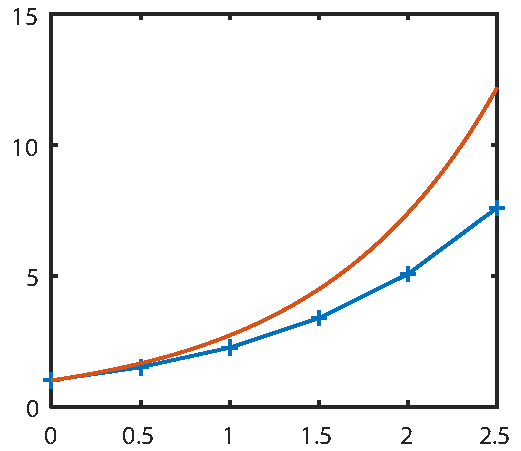
\includegraphics[width=7cm]{./figures/OdeMid.pdf}
\caption{欧拉法数值解(蓝)和解析解(红)} \label{OdeMid_fig1}
\end{figure}

由“”%词条未完成
我们知道该方程的解析解为 $y = \E^{t}$. 对比数值解和解析解, 不难分析出误差产生的原因: 我们仅用每段步长区间左端的导数预测整个区间的曲线增量. 如果我们能利用每个区间的中点的导数计算计算整个区间的增量, 这个预测将会比欧拉法更精确.

考虑微分方程 $y'(t) = f(y, t)$ 在区间 $[t_n, t_{n+1}]$ 的曲线, 若我们已知区间左端的函数值为 $y_n$, 我们可以先用微分近似估计曲线中点的函数值为
\begin{equation}
y\left(t_n + \frac h2\right) = y_n + \frac h2 f(y_n, t_n)
\end{equation}
然后再求出这个近似中点的导数为
\begin{equation}
y'\left(t_n + \frac h2\right) = f\left[y_n + \frac h2 f(t_n, y_n), t_n + \frac h2\right]
\end{equation}
最后我们利用这个导数估算该区间的曲线增量
\begin{equation}
y_{n+1} = y_n + hy'\left(t_n + \frac h2\right) = y_n + h f\left[y_n + \frac h2 f(t_n, y_n), t_n + \frac h2\right]
\end{equation}
这就是解常微分方程的\textbf{中点法}.

我们再来用中点法取同样的步长计算\autoref{OdeMid_eq1}, 结果如\autoref{OdeMid_fig2} 所示.

\begin{figure}[ht]
\centering
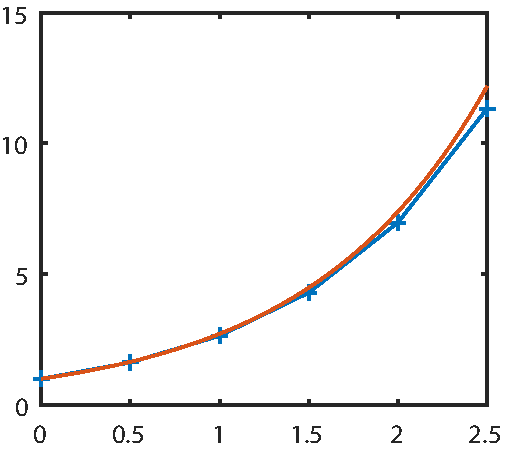
\includegraphics[width=7cm]{./figures/OdeMid2.pdf}
\caption{欧拉法数值解(蓝)和解析解(红)} \label{OdeMid_fig2}
\end{figure}

可见虽然中点法每一步的计算过程比欧拉法稍微复杂一些, 但精度却大大地提高了. 

中点法同样适用于微分方程组, 例如对于常微分方程组
\begin{equation}\leftgroup{
x'(t) &= f(x, y, t)\\
y'(t) &= g(x, y, t)
}\end{equation}
首先计算近似中点为
\begin{equation}\leftgroup{
x_{n+1/2} &= x_n + h f(x_n, y_n, t_n)\\
y_{n+1/2} &= y_n + h g(x_n, y_n, t_n)
}\end{equation}
然后有
\begin{equation}\leftgroup{
x_{n+1} &= x_n + h f\left(x_{n+1/2}, y_{n+1/2}, \frac h2\right)\\
y_{n+1} &= y_n + h g\left(x_{n+1/2}, y_{n+1/2}, \frac h2\right)
}\end{equation}

\subsection{例程}

% 设置参数
N = 6;
h = 0.5;
t = linspace(0, (N-1)*h, N); % 自变量
t0 = linspace(0, (N-1)*h, 100); % 用于画图

% 欧拉法
y = zeros(1,N); % 预赋值
y(1) = 1; % 初值
for ii = 1:N-1
    y(ii+1) = y(ii) + h*y(ii);
end

% 画图
figure;
plot(x,y,'+-');
hold on;
plot(t0, exp(t0));

%中点法
y = zeros(1,N);
y(1) = 1;
for ii = 1:N-1
    y(ii+1) = y(ii) + h*(y(ii) + 0.5*h*y(ii));
end

% 画图
figure;
plot(x,y,'+-');
hold on;
plot(x0, exp(x0));




